% Options for packages loaded elsewhere
\PassOptionsToPackage{unicode}{hyperref}
\PassOptionsToPackage{hyphens}{url}
\PassOptionsToPackage{dvipsnames,svgnames,x11names}{xcolor}
%
\documentclass[
  a4paper,
  DIV=11,
  numbers=noendperiod]{scrreprt}

\usepackage{amsmath,amssymb}
\usepackage{iftex}
\ifPDFTeX
  \usepackage[T1]{fontenc}
  \usepackage[utf8]{inputenc}
  \usepackage{textcomp} % provide euro and other symbols
\else % if luatex or xetex
  \usepackage{unicode-math}
  \defaultfontfeatures{Scale=MatchLowercase}
  \defaultfontfeatures[\rmfamily]{Ligatures=TeX,Scale=1}
\fi
\usepackage{lmodern}
\ifPDFTeX\else  
    % xetex/luatex font selection
\fi
% Use upquote if available, for straight quotes in verbatim environments
\IfFileExists{upquote.sty}{\usepackage{upquote}}{}
\IfFileExists{microtype.sty}{% use microtype if available
  \usepackage[]{microtype}
  \UseMicrotypeSet[protrusion]{basicmath} % disable protrusion for tt fonts
}{}
\usepackage{xcolor}
\setlength{\emergencystretch}{3em} % prevent overfull lines
\setcounter{secnumdepth}{2}
% Make \paragraph and \subparagraph free-standing
\ifx\paragraph\undefined\else
  \let\oldparagraph\paragraph
  \renewcommand{\paragraph}[1]{\oldparagraph{#1}\mbox{}}
\fi
\ifx\subparagraph\undefined\else
  \let\oldsubparagraph\subparagraph
  \renewcommand{\subparagraph}[1]{\oldsubparagraph{#1}\mbox{}}
\fi


\providecommand{\tightlist}{%
  \setlength{\itemsep}{0pt}\setlength{\parskip}{0pt}}\usepackage{longtable,booktabs,array}
\usepackage{calc} % for calculating minipage widths
% Correct order of tables after \paragraph or \subparagraph
\usepackage{etoolbox}
\makeatletter
\patchcmd\longtable{\par}{\if@noskipsec\mbox{}\fi\par}{}{}
\makeatother
% Allow footnotes in longtable head/foot
\IfFileExists{footnotehyper.sty}{\usepackage{footnotehyper}}{\usepackage{footnote}}
\makesavenoteenv{longtable}
\usepackage{graphicx}
\makeatletter
\def\maxwidth{\ifdim\Gin@nat@width>\linewidth\linewidth\else\Gin@nat@width\fi}
\def\maxheight{\ifdim\Gin@nat@height>\textheight\textheight\else\Gin@nat@height\fi}
\makeatother
% Scale images if necessary, so that they will not overflow the page
% margins by default, and it is still possible to overwrite the defaults
% using explicit options in \includegraphics[width, height, ...]{}
\setkeys{Gin}{width=\maxwidth,height=\maxheight,keepaspectratio}
% Set default figure placement to htbp
\makeatletter
\def\fps@figure{htbp}
\makeatother
\newlength{\cslhangindent}
\setlength{\cslhangindent}{1.5em}
\newlength{\csllabelwidth}
\setlength{\csllabelwidth}{3em}
\newlength{\cslentryspacingunit} % times entry-spacing
\setlength{\cslentryspacingunit}{\parskip}
\newenvironment{CSLReferences}[2] % #1 hanging-ident, #2 entry spacing
 {% don't indent paragraphs
  \setlength{\parindent}{0pt}
  % turn on hanging indent if param 1 is 1
  \ifodd #1
  \let\oldpar\par
  \def\par{\hangindent=\cslhangindent\oldpar}
  \fi
  % set entry spacing
  \setlength{\parskip}{#2\cslentryspacingunit}
 }%
 {}
\usepackage{calc}
\newcommand{\CSLBlock}[1]{#1\hfill\break}
\newcommand{\CSLLeftMargin}[1]{\parbox[t]{\csllabelwidth}{#1}}
\newcommand{\CSLRightInline}[1]{\parbox[t]{\linewidth - \csllabelwidth}{#1}\break}
\newcommand{\CSLIndent}[1]{\hspace{\cslhangindent}#1}

\usepackage{amsmath}
\KOMAoption{captions}{tableheading}
\makeatletter
\makeatother
\makeatletter
\@ifpackageloaded{bookmark}{}{\usepackage{bookmark}}
\makeatother
\makeatletter
\@ifpackageloaded{caption}{}{\usepackage{caption}}
\AtBeginDocument{%
\ifdefined\contentsname
  \renewcommand*\contentsname{Table of contents}
\else
  \newcommand\contentsname{Table of contents}
\fi
\ifdefined\listfigurename
  \renewcommand*\listfigurename{List of Figures}
\else
  \newcommand\listfigurename{List of Figures}
\fi
\ifdefined\listtablename
  \renewcommand*\listtablename{List of Tables}
\else
  \newcommand\listtablename{List of Tables}
\fi
\ifdefined\figurename
  \renewcommand*\figurename{Figure}
\else
  \newcommand\figurename{Figure}
\fi
\ifdefined\tablename
  \renewcommand*\tablename{Table}
\else
  \newcommand\tablename{Table}
\fi
}
\@ifpackageloaded{float}{}{\usepackage{float}}
\floatstyle{ruled}
\@ifundefined{c@chapter}{\newfloat{codelisting}{h}{lop}}{\newfloat{codelisting}{h}{lop}[chapter]}
\floatname{codelisting}{Listing}
\newcommand*\listoflistings{\listof{codelisting}{List of Listings}}
\makeatother
\makeatletter
\@ifpackageloaded{caption}{}{\usepackage{caption}}
\@ifpackageloaded{subcaption}{}{\usepackage{subcaption}}
\makeatother
\makeatletter
\@ifpackageloaded{tcolorbox}{}{\usepackage[skins,breakable]{tcolorbox}}
\makeatother
\makeatletter
\@ifundefined{shadecolor}{\definecolor{shadecolor}{rgb}{.97, .97, .97}}
\makeatother
\makeatletter
\makeatother
\makeatletter
\makeatother
\ifLuaTeX
  \usepackage{selnolig}  % disable illegal ligatures
\fi
\IfFileExists{bookmark.sty}{\usepackage{bookmark}}{\usepackage{hyperref}}
\IfFileExists{xurl.sty}{\usepackage{xurl}}{} % add URL line breaks if available
\urlstyle{same} % disable monospaced font for URLs
\hypersetup{
  pdftitle={Ambiguity attitudes and surprises:},
  pdfauthor={Aljoscha Minnich; Hauke Roggenkamp; Andreas Lange},
  colorlinks=true,
  linkcolor={blue},
  filecolor={Maroon},
  citecolor={Blue},
  urlcolor={Blue},
  pdfcreator={LaTeX via pandoc}}

\title{Ambiguity attitudes and surprises:}
\usepackage{etoolbox}
\makeatletter
\providecommand{\subtitle}[1]{% add subtitle to \maketitle
  \apptocmd{\@title}{\par {\large #1 \par}}{}{}
}
\makeatother
\subtitle{Computational reproduction}
\author{Aljoscha Minnich \and Hauke Roggenkamp \and Andreas Lange}
\date{2024-07-15}

\begin{document}
\maketitle
\ifdefined\Shaded\renewenvironment{Shaded}{\begin{tcolorbox}[breakable, frame hidden, sharp corners, enhanced, interior hidden, boxrule=0pt, borderline west={3pt}{0pt}{shadecolor}]}{\end{tcolorbox}}\fi

\renewcommand*\contentsname{Table of contents}
{
\hypersetup{linkcolor=}
\setcounter{tocdepth}{2}
\tableofcontents
}
\bookmarksetup{startatroot}

\hypertarget{preface}{%
\chapter*{Preface}\label{preface}}
\addcontentsline{toc}{chapter}{Preface}

\markboth{Preface}{Preface}

This document explains and shows how to reproduce the figures and tables
displayed in our paper using a literate programming approach (Knuth
1984).

\bookmarksetup{startatroot}

\hypertarget{pre-processing}{%
\chapter{Pre-Processing}\label{pre-processing}}

This document explains how to process the raw data into a tidy format.
We assume familiarity with our paper \emph{(Ambiguity attitudes and
surprises)} and recommend to also read Baillon et al. (2018) to better
understand the method we apply in this document.

\hypertarget{install-packages}{%
\section{Install Packages}\label{install-packages}}

We install the following packages using the \texttt{groundhog} package
manager to increase computational reproducibility.

\hypertarget{read-data}{%
\section{Read Data}\label{read-data}}

We read two data files. First, \texttt{raw}, that is, a raw data set
containing all variables defined in (Chen, Schonger, and Wickens 2016).
This is the data we are most interested in as it contains all of our
behavioral measures (see Baillon et al. 2018) and
self-reports.\footnote{Note that we removed three variables to maintain
  anonymity of participants: their reported zip codes as well as two
  open-text fields rather unrelated to this study.} Second,
\texttt{time\_spent} describes how much time each participant spent on a
given page of the online experiment.

\hypertarget{exclusion}{%
\section{Exclusion}\label{exclusion}}

We drop several rows of the \texttt{raw} data based on two conditions:

\begin{enumerate}
\def\labelenumi{\arabic{enumi}.}
\tightlist
\item
  We only want to keep observations that finished the survey (i.e., they
  reached the \texttt{\_max\_page\_index}).
\item
  We want to exclude rows created during testing and only keep those,
  where the \texttt{participant.label} is a 32-character alpha-numeric
  string provided by the sample provider.
\end{enumerate}

The result is assigned to a data.tabled called \texttt{DT}.

\hypertarget{primary-outcomes}{%
\section{Primary Outcomes}\label{primary-outcomes}}

Following Baillon et al. (2018), we study two indices capturing
ambiguity attitudes:

\[
b=1-\overline{m_s}-\overline{m_c} \qquad \qquad a= 3 \times (\frac{1}{3} -(\overline{m_c}-\overline{m_s})).
\]

Index \emph{b} captures the \emph{ambiguity aversion} and ranges from -1
to 1. A negative \emph{b} can be interpreted as ambiguity seeking, while
a positive \emph{b} refers to ambiguity aversion: in fact, for expected
utility maximizers, i.e., ambiguity-neutral decision makers, the
probability equivalents of an event and its complement adds to 1 such
that the index takes value 0.

Index \emph{a} is referred to as the \emph{ambiguity-generating
insensitivity index}. It measures to what extent the matching
probabilities converge towards 50\%. Again, it takes value 0 under
ambiguity neutrality as \(\overline{m_s} = \frac{1}{3}\) and
\(\overline{m_c} = \frac{2}{3}\). Positive values of \emph{a} indicate
overweighted low probabilities and underweighted high probabilities,
reflecting relative insensitivity. In contrast, negative values of
\emph{a} indicate underweighted low probabilities and overweighted high
probabilities (Anantanasuwong et al. 2019).

For the sake of convenience, we start to compute these indices by
dropping all the columns that we do not need for this step and keep the
\texttt{participant.id} to match the data later on. To do so, we use a
regex.

We then rename the two treatment variables, \texttt{surprise} and
\texttt{communication}:

\begin{longtable}[]{@{}
  >{\raggedright\arraybackslash}p{(\columnwidth - 52\tabcolsep) * \real{0.0366}}
  >{\raggedright\arraybackslash}p{(\columnwidth - 52\tabcolsep) * \real{0.0155}}
  >{\raggedleft\arraybackslash}p{(\columnwidth - 52\tabcolsep) * \real{0.0421}}
  >{\raggedright\arraybackslash}p{(\columnwidth - 52\tabcolsep) * \real{0.0355}}
  >{\raggedleft\arraybackslash}p{(\columnwidth - 52\tabcolsep) * \real{0.0421}}
  >{\raggedright\arraybackslash}p{(\columnwidth - 52\tabcolsep) * \real{0.0355}}
  >{\raggedleft\arraybackslash}p{(\columnwidth - 52\tabcolsep) * \real{0.0421}}
  >{\raggedright\arraybackslash}p{(\columnwidth - 52\tabcolsep) * \real{0.0355}}
  >{\raggedleft\arraybackslash}p{(\columnwidth - 52\tabcolsep) * \real{0.0421}}
  >{\raggedright\arraybackslash}p{(\columnwidth - 52\tabcolsep) * \real{0.0355}}
  >{\raggedleft\arraybackslash}p{(\columnwidth - 52\tabcolsep) * \real{0.0421}}
  >{\raggedright\arraybackslash}p{(\columnwidth - 52\tabcolsep) * \real{0.0355}}
  >{\raggedleft\arraybackslash}p{(\columnwidth - 52\tabcolsep) * \real{0.0421}}
  >{\raggedright\arraybackslash}p{(\columnwidth - 52\tabcolsep) * \real{0.0355}}
  >{\raggedleft\arraybackslash}p{(\columnwidth - 52\tabcolsep) * \real{0.0421}}
  >{\raggedright\arraybackslash}p{(\columnwidth - 52\tabcolsep) * \real{0.0355}}
  >{\raggedleft\arraybackslash}p{(\columnwidth - 52\tabcolsep) * \real{0.0421}}
  >{\raggedright\arraybackslash}p{(\columnwidth - 52\tabcolsep) * \real{0.0355}}
  >{\raggedleft\arraybackslash}p{(\columnwidth - 52\tabcolsep) * \real{0.0421}}
  >{\raggedright\arraybackslash}p{(\columnwidth - 52\tabcolsep) * \real{0.0355}}
  >{\raggedleft\arraybackslash}p{(\columnwidth - 52\tabcolsep) * \real{0.0432}}
  >{\raggedright\arraybackslash}p{(\columnwidth - 52\tabcolsep) * \real{0.0366}}
  >{\raggedleft\arraybackslash}p{(\columnwidth - 52\tabcolsep) * \real{0.0432}}
  >{\raggedright\arraybackslash}p{(\columnwidth - 52\tabcolsep) * \real{0.0366}}
  >{\raggedleft\arraybackslash}p{(\columnwidth - 52\tabcolsep) * \real{0.0432}}
  >{\raggedright\arraybackslash}p{(\columnwidth - 52\tabcolsep) * \real{0.0366}}
  >{\raggedright\arraybackslash}p{(\columnwidth - 52\tabcolsep) * \real{0.0100}}@{}}
\toprule\noalign{}
\begin{minipage}[b]{\linewidth}\raggedright
participant.label
\end{minipage} & \begin{minipage}[b]{\linewidth}\raggedright
communication
\end{minipage} & \begin{minipage}[b]{\linewidth}\raggedleft
Baillon.1.player.matching\_probability
\end{minipage} & \begin{minipage}[b]{\linewidth}\raggedright
Baillon.1.player.event\_decision
\end{minipage} & \begin{minipage}[b]{\linewidth}\raggedleft
Baillon.2.player.matching\_probability
\end{minipage} & \begin{minipage}[b]{\linewidth}\raggedright
Baillon.2.player.event\_decision
\end{minipage} & \begin{minipage}[b]{\linewidth}\raggedleft
Baillon.3.player.matching\_probability
\end{minipage} & \begin{minipage}[b]{\linewidth}\raggedright
Baillon.3.player.event\_decision
\end{minipage} & \begin{minipage}[b]{\linewidth}\raggedleft
Baillon.4.player.matching\_probability
\end{minipage} & \begin{minipage}[b]{\linewidth}\raggedright
Baillon.4.player.event\_decision
\end{minipage} & \begin{minipage}[b]{\linewidth}\raggedleft
Baillon.5.player.matching\_probability
\end{minipage} & \begin{minipage}[b]{\linewidth}\raggedright
Baillon.5.player.event\_decision
\end{minipage} & \begin{minipage}[b]{\linewidth}\raggedleft
Baillon.6.player.matching\_probability
\end{minipage} & \begin{minipage}[b]{\linewidth}\raggedright
Baillon.6.player.event\_decision
\end{minipage} & \begin{minipage}[b]{\linewidth}\raggedleft
Baillon.7.player.matching\_probability
\end{minipage} & \begin{minipage}[b]{\linewidth}\raggedright
Baillon.7.player.event\_decision
\end{minipage} & \begin{minipage}[b]{\linewidth}\raggedleft
Baillon.8.player.matching\_probability
\end{minipage} & \begin{minipage}[b]{\linewidth}\raggedright
Baillon.8.player.event\_decision
\end{minipage} & \begin{minipage}[b]{\linewidth}\raggedleft
Baillon.9.player.matching\_probability
\end{minipage} & \begin{minipage}[b]{\linewidth}\raggedright
Baillon.9.player.event\_decision
\end{minipage} & \begin{minipage}[b]{\linewidth}\raggedleft
Baillon.10.player.matching\_probability
\end{minipage} & \begin{minipage}[b]{\linewidth}\raggedright
Baillon.10.player.event\_decision
\end{minipage} & \begin{minipage}[b]{\linewidth}\raggedleft
Baillon.11.player.matching\_probability
\end{minipage} & \begin{minipage}[b]{\linewidth}\raggedright
Baillon.11.player.event\_decision
\end{minipage} & \begin{minipage}[b]{\linewidth}\raggedleft
Baillon.12.player.matching\_probability
\end{minipage} & \begin{minipage}[b]{\linewidth}\raggedright
Baillon.12.player.event\_decision
\end{minipage} & \begin{minipage}[b]{\linewidth}\raggedright
surprise
\end{minipage} \\
\midrule\noalign{}
\endhead
\bottomrule\noalign{}
\endlastfoot
0e379132b6dab27b63921c941312840f & interval & 67 & E13 & 67 & E12 & 34 &
E1 & 67 & E23 & 34 & E3 & 34 & E2 & 66 & E13 & 67 & E12 & 34 & E1 & 67 &
E23 & 34 & E3 & 34 & E2 & TRUE \\
ca48f818955f9a22b31d290dc2a28723 & both & 70 & E23 & 70 & E12 & 40 & E2
& 7 & E13 & 40 & E3 & 40 & E1 & 70 & E23 & 70 & E12 & 40 & E2 & 70 & E13
& 40 & E3 & 40 & E1 & TRUE \\
6ccf7afc080efce8a5d08fe2b3547b3e & interval & 45 & E23 & 55 & E2 & 45 &
E12 & 40 & E3 & 35 & E13 & 55 & E1 & 30 & E23 & 60 & E2 & 40 & E12 & 55
& E3 & 60 & E13 & 65 & E1 & FALSE \\
50a040bc4e4e9266a0f40b85fd4e4d0e & both & 51 & E12 & 51 & E3 & 51 & E2 &
67 & E13 & 51 & E1 & 67 & E23 & 80 & E12 & 67 & E3 & 80 & E2 & 67 & E13
& 51 & E1 & 67 & E23 & TRUE \\
c1709a48b7d3e4a55aeaf6feb55eaf69 & both & 50 & E2 & 55 & E1 & 50 & E12 &
45 & E13 & 60 & E3 & 58 & E23 & 45 & E2 & 47 & E1 & 50 & E12 & 55 & E13
& 40 & E3 & 52 & E23 & FALSE \\
79c8aa8a670d96b4afb54af9fca6e6a8 & both & 45 & E1 & 56 & E12 & 46 & E2 &
63 & E23 & 58 & E13 & 47 & E3 & 43 & E1 & 54 & E12 & 49 & E2 & 67 & E23
& 59 & E13 & 45 & E3 & FALSE \\
0c42458206b38f6b28125c23ac8fbd8b & interval & 70 & E13 & 67 & E12 & 65 &
E3 & 80 & E23 & 50 & E2 & 45 & E1 & 50 & E13 & 50 & E12 & 50 & E3 & 67 &
E23 & 65 & E2 & 30 & E1 & FALSE \\
\end{longtable}

We then use \texttt{data.table::melt()} to create a long table, create a
\texttt{stage} as well as a \texttt{treated} variable that express
treatment status. In addition, we correct matching probabilities
equaling 101. Because the stated number of winning balls indicates the
minimum number of balls such that the lottery is preferred, we subtract
0.5 from the selected values to specify the matching probability
(indifference point)

\begin{longtable}[]{@{}
  >{\raggedright\arraybackslash}p{(\columnwidth - 14\tabcolsep) * \real{0.3402}}
  >{\raggedright\arraybackslash}p{(\columnwidth - 14\tabcolsep) * \real{0.0928}}
  >{\raggedright\arraybackslash}p{(\columnwidth - 14\tabcolsep) * \real{0.1443}}
  >{\raggedleft\arraybackslash}p{(\columnwidth - 14\tabcolsep) * \real{0.0722}}
  >{\raggedleft\arraybackslash}p{(\columnwidth - 14\tabcolsep) * \real{0.1443}}
  >{\raggedright\arraybackslash}p{(\columnwidth - 14\tabcolsep) * \real{0.0619}}
  >{\raggedleft\arraybackslash}p{(\columnwidth - 14\tabcolsep) * \real{0.0619}}
  >{\raggedright\arraybackslash}p{(\columnwidth - 14\tabcolsep) * \real{0.0825}}@{}}
\toprule\noalign{}
\begin{minipage}[b]{\linewidth}\raggedright
participant.label
\end{minipage} & \begin{minipage}[b]{\linewidth}\raggedright
surprise
\end{minipage} & \begin{minipage}[b]{\linewidth}\raggedright
communication
\end{minipage} & \begin{minipage}[b]{\linewidth}\raggedleft
period
\end{minipage} & \begin{minipage}[b]{\linewidth}\raggedleft
matching\_prob
\end{minipage} & \begin{minipage}[b]{\linewidth}\raggedright
event
\end{minipage} & \begin{minipage}[b]{\linewidth}\raggedleft
stage
\end{minipage} & \begin{minipage}[b]{\linewidth}\raggedright
treated
\end{minipage} \\
\midrule\noalign{}
\endhead
\bottomrule\noalign{}
\endlastfoot
0e379132b6dab27b63921c941312840f & TRUE & interval & 1 & 66.5 & E13 & 1
& FALSE \\
ca48f818955f9a22b31d290dc2a28723 & TRUE & both & 1 & 69.5 & E23 & 1 &
FALSE \\
6ccf7afc080efce8a5d08fe2b3547b3e & FALSE & interval & 1 & 44.5 & E23 & 1
& FALSE \\
50a040bc4e4e9266a0f40b85fd4e4d0e & TRUE & both & 1 & 50.5 & E12 & 1 &
FALSE \\
c1709a48b7d3e4a55aeaf6feb55eaf69 & FALSE & both & 1 & 49.5 & E2 & 1 &
FALSE \\
79c8aa8a670d96b4afb54af9fca6e6a8 & FALSE & both & 1 & 44.5 & E1 & 1 &
FALSE \\
0c42458206b38f6b28125c23ac8fbd8b & FALSE & interval & 1 & 69.5 & E13 & 1
& FALSE \\
\end{longtable}

Next, we reshape that table once more and bring it to a wide format
using \texttt{data.table::dcast()} and call the result
\texttt{event\_data}.

We now change the data class of \texttt{communication} and make it a
factor.

Finally, we create the indices we are interested in (mainly \texttt{b}
and \texttt{a}) as well as the Euclidyan distance (\texttt{ed}) between
matching probabilities prior to and after treatment.

\begin{longtable}[]{@{}
  >{\raggedright\arraybackslash}p{(\columnwidth - 30\tabcolsep) * \real{0.2260}}
  >{\raggedright\arraybackslash}p{(\columnwidth - 30\tabcolsep) * \real{0.0616}}
  >{\raggedright\arraybackslash}p{(\columnwidth - 30\tabcolsep) * \real{0.0959}}
  >{\raggedleft\arraybackslash}p{(\columnwidth - 30\tabcolsep) * \real{0.0411}}
  >{\raggedright\arraybackslash}p{(\columnwidth - 30\tabcolsep) * \real{0.0548}}
  >{\raggedleft\arraybackslash}p{(\columnwidth - 30\tabcolsep) * \real{0.0342}}
  >{\raggedleft\arraybackslash}p{(\columnwidth - 30\tabcolsep) * \real{0.0342}}
  >{\raggedleft\arraybackslash}p{(\columnwidth - 30\tabcolsep) * \real{0.0342}}
  >{\raggedleft\arraybackslash}p{(\columnwidth - 30\tabcolsep) * \real{0.0342}}
  >{\raggedleft\arraybackslash}p{(\columnwidth - 30\tabcolsep) * \real{0.0342}}
  >{\raggedleft\arraybackslash}p{(\columnwidth - 30\tabcolsep) * \real{0.0342}}
  >{\raggedleft\arraybackslash}p{(\columnwidth - 30\tabcolsep) * \real{0.0685}}
  >{\raggedleft\arraybackslash}p{(\columnwidth - 30\tabcolsep) * \real{0.0685}}
  >{\raggedleft\arraybackslash}p{(\columnwidth - 30\tabcolsep) * \real{0.0753}}
  >{\raggedleft\arraybackslash}p{(\columnwidth - 30\tabcolsep) * \real{0.0411}}
  >{\raggedleft\arraybackslash}p{(\columnwidth - 30\tabcolsep) * \real{0.0616}}@{}}
\toprule\noalign{}
\begin{minipage}[b]{\linewidth}\raggedright
participant.label
\end{minipage} & \begin{minipage}[b]{\linewidth}\raggedright
surprise
\end{minipage} & \begin{minipage}[b]{\linewidth}\raggedright
communication
\end{minipage} & \begin{minipage}[b]{\linewidth}\raggedleft
stage
\end{minipage} & \begin{minipage}[b]{\linewidth}\raggedright
treated
\end{minipage} & \begin{minipage}[b]{\linewidth}\raggedleft
E1
\end{minipage} & \begin{minipage}[b]{\linewidth}\raggedleft
E12
\end{minipage} & \begin{minipage}[b]{\linewidth}\raggedleft
E13
\end{minipage} & \begin{minipage}[b]{\linewidth}\raggedleft
E2
\end{minipage} & \begin{minipage}[b]{\linewidth}\raggedleft
E23
\end{minipage} & \begin{minipage}[b]{\linewidth}\raggedleft
E3
\end{minipage} & \begin{minipage}[b]{\linewidth}\raggedleft
mc
\end{minipage} & \begin{minipage}[b]{\linewidth}\raggedleft
ms
\end{minipage} & \begin{minipage}[b]{\linewidth}\raggedleft
b
\end{minipage} & \begin{minipage}[b]{\linewidth}\raggedleft
a
\end{minipage} & \begin{minipage}[b]{\linewidth}\raggedleft
ed
\end{minipage} \\
\midrule\noalign{}
\endhead
\bottomrule\noalign{}
\endlastfoot
01c4f6a51f1a756640eaa8c97302edc8 & FALSE & both & 1 & FALSE & 49.5 &
49.5 & 69.5 & 33.5 & 66.5 & 35.5 & 0.6183333 & 0.3950000 & -0.0133333 &
0.33 & 60.38212 \\
01c4f6a51f1a756640eaa8c97302edc8 & FALSE & both & 2 & TRUE & 9.5 & 74.5
& 39.5 & 49.5 & 69.5 & 19.5 & 0.6116667 & 0.2616667 & 0.1266667 & -0.05
& 60.38212 \\
026c74f9a6c56e375ee0f248c2a13ff0 & FALSE & both & 1 & FALSE & 33.5 &
66.5 & 66.5 & 33.5 & 66.5 & 33.5 & 0.6650000 & 0.3350000 & 0.0000000 &
0.01 & 0.00000 \\
026c74f9a6c56e375ee0f248c2a13ff0 & FALSE & both & 2 & TRUE & 33.5 & 66.5
& 66.5 & 33.5 & 66.5 & 33.5 & 0.6650000 & 0.3350000 & 0.0000000 & 0.01 &
0.00000 \\
0403e88278229630e892f8887fe351a8 & FALSE & both & 1 & FALSE & 59.5 &
74.5 & 49.5 & 49.5 & 64.5 & 69.5 & 0.6283333 & 0.5950000 & -0.2233333 &
0.90 & 38.07887 \\
0403e88278229630e892f8887fe351a8 & FALSE & both & 2 & TRUE & 49.5 & 49.5
& 69.5 & 49.5 & 79.5 & 59.5 & 0.6616667 & 0.5283333 & -0.1900000 & 0.60
& 38.07887 \\
041ed5ab429aeb34d1c0c8da5d3d2ec8 & FALSE & both & 1 & FALSE & 84.5 &
49.5 & 49.5 & 49.5 & 49.5 & 39.5 & 0.4950000 & 0.5783333 & -0.0733333 &
1.25 & 40.62019 \\
\end{longtable}

\hypertarget{self-reports}{%
\section{Self-Reports}\label{self-reports}}

For the sake of clarity, we select self-reported columns as well as the
\texttt{participant.label} while processing the self-reported data.
Doing so, we exploit that all self-reports were elicited in the so
called \texttt{Outro} app, which is why we can select the corresponding
columns using oTree's naming convention.

To increase clarity further, we drop irrelevant information from oTree's
naming convention (e.g., replace the name of
\texttt{Outro.1.player.Family} with \emph{``family''}).

Next, we dichotomize several self-reports using a median split.

In addition, we hard-code some variables.

\begin{longtable}[]{@{}
  >{\raggedright\arraybackslash}p{(\columnwidth - 32\tabcolsep) * \real{0.1289}}
  >{\raggedright\arraybackslash}p{(\columnwidth - 32\tabcolsep) * \real{0.1133}}
  >{\raggedright\arraybackslash}p{(\columnwidth - 32\tabcolsep) * \real{0.0547}}
  >{\raggedright\arraybackslash}p{(\columnwidth - 32\tabcolsep) * \real{0.0391}}
  >{\raggedright\arraybackslash}p{(\columnwidth - 32\tabcolsep) * \real{0.0391}}
  >{\raggedright\arraybackslash}p{(\columnwidth - 32\tabcolsep) * \real{0.0469}}
  >{\raggedright\arraybackslash}p{(\columnwidth - 32\tabcolsep) * \real{0.0273}}
  >{\raggedright\arraybackslash}p{(\columnwidth - 32\tabcolsep) * \real{0.0586}}
  >{\raggedright\arraybackslash}p{(\columnwidth - 32\tabcolsep) * \real{0.0469}}
  >{\raggedright\arraybackslash}p{(\columnwidth - 32\tabcolsep) * \real{0.0312}}
  >{\raggedright\arraybackslash}p{(\columnwidth - 32\tabcolsep) * \real{0.0430}}
  >{\raggedright\arraybackslash}p{(\columnwidth - 32\tabcolsep) * \real{0.0664}}
  >{\raggedright\arraybackslash}p{(\columnwidth - 32\tabcolsep) * \real{0.0430}}
  >{\raggedright\arraybackslash}p{(\columnwidth - 32\tabcolsep) * \real{0.0703}}
  >{\raggedright\arraybackslash}p{(\columnwidth - 32\tabcolsep) * \real{0.0703}}
  >{\raggedright\arraybackslash}p{(\columnwidth - 32\tabcolsep) * \real{0.0547}}
  >{\raggedright\arraybackslash}p{(\columnwidth - 32\tabcolsep) * \real{0.0664}}@{}}
\toprule\noalign{}
\begin{minipage}[b]{\linewidth}\raggedright
participant.label
\end{minipage} & \begin{minipage}[b]{\linewidth}\raggedright
participant.time\_started\_utc
\end{minipage} & \begin{minipage}[b]{\linewidth}\raggedright
comprehension
\end{minipage} & \begin{minipage}[b]{\linewidth}\raggedright
age\_18\_34
\end{minipage} & \begin{minipage}[b]{\linewidth}\raggedright
age\_35\_52
\end{minipage} & \begin{minipage}[b]{\linewidth}\raggedright
age\_53\_plus
\end{minipage} & \begin{minipage}[b]{\linewidth}\raggedright
female
\end{minipage} & \begin{minipage}[b]{\linewidth}\raggedright
high\_education
\end{minipage} & \begin{minipage}[b]{\linewidth}\raggedright
high\_income
\end{minipage} & \begin{minipage}[b]{\linewidth}\raggedright
married
\end{minipage} & \begin{minipage}[b]{\linewidth}\raggedright
parentship
\end{minipage} & \begin{minipage}[b]{\linewidth}\raggedright
high\_temperature
\end{minipage} & \begin{minipage}[b]{\linewidth}\raggedright
high\_usage
\end{minipage} & \begin{minipage}[b]{\linewidth}\raggedright
high\_general\_risk
\end{minipage} & \begin{minipage}[b]{\linewidth}\raggedright
high\_weather\_risk
\end{minipage} & \begin{minipage}[b]{\linewidth}\raggedright
high\_accuracy
\end{minipage} & \begin{minipage}[b]{\linewidth}\raggedright
high\_credibility
\end{minipage} \\
\midrule\noalign{}
\endhead
\bottomrule\noalign{}
\endlastfoot
0e379132b6dab27b63921c941312840f & 2021-09-02 11:06:03 & rather yes &
FALSE & TRUE & FALSE & TRUE & FALSE & FALSE & FALSE & FALSE & FALSE &
TRUE & FALSE & FALSE & TRUE & FALSE \\
ca48f818955f9a22b31d290dc2a28723 & 2021-09-02 11:22:18 & rather yes &
TRUE & FALSE & FALSE & TRUE & FALSE & TRUE & TRUE & FALSE & TRUE & FALSE
& TRUE & TRUE & TRUE & TRUE \\
6ccf7afc080efce8a5d08fe2b3547b3e & 2021-09-02 11:25:21 & rather yes &
FALSE & TRUE & FALSE & FALSE & TRUE & TRUE & TRUE & FALSE & TRUE & FALSE
& TRUE & TRUE & TRUE & TRUE \\
50a040bc4e4e9266a0f40b85fd4e4d0e & 2021-09-02 11:36:03 & rather yes &
FALSE & TRUE & FALSE & TRUE & TRUE & FALSE & FALSE & TRUE & FALSE &
FALSE & FALSE & TRUE & FALSE & FALSE \\
c1709a48b7d3e4a55aeaf6feb55eaf69 & 2021-09-02 11:47:01 & rather not &
FALSE & FALSE & TRUE & FALSE & FALSE & TRUE & TRUE & TRUE & TRUE & FALSE
& FALSE & FALSE & TRUE & FALSE \\
79c8aa8a670d96b4afb54af9fca6e6a8 & 2021-09-02 11:52:48 & rather yes &
FALSE & FALSE & TRUE & TRUE & TRUE & TRUE & FALSE & FALSE & TRUE & TRUE
& TRUE & FALSE & FALSE & TRUE \\
0c42458206b38f6b28125c23ac8fbd8b & 2021-09-02 12:08:26 & yes & FALSE &
TRUE & FALSE & FALSE & TRUE & TRUE & TRUE & TRUE & TRUE & TRUE & TRUE &
TRUE & TRUE & FALSE \\
\end{longtable}

\hypertarget{comprehension-questions}{%
\section{Comprehension Questions}\label{comprehension-questions}}

For robustness checks, we subset participants, who did answer the
comprehension questions correctly at their first try. These information
are stored in the \texttt{Intro} app, which we now select and rename
before we merge it with the remaining data later on.

\hypertarget{time-spent}{%
\section{Time Spent}\label{time-spent}}

Next, we calculate how much time a participant spent on a given page. To
do so, we subtract time stamps which were recorded whenever a page was
submitted. The difference of two subsequent time stamps
(\texttt{time\_spent\_on\_page}) therefore tells us how much time a
participant spent on a given page.

We calculate the \texttt{time\_spent\_on\_page} metric, store it in a
data table \texttt{duration} and add a \texttt{participant.label} column
that is not inherent to the available \texttt{time\_spent} data (and
which we use as the key ID to match data).

\begin{longtable}[]{@{}
  >{\raggedright\arraybackslash}p{(\columnwidth - 16\tabcolsep) * \real{0.0833}}
  >{\raggedright\arraybackslash}p{(\columnwidth - 16\tabcolsep) * \real{0.1090}}
  >{\raggedright\arraybackslash}p{(\columnwidth - 16\tabcolsep) * \real{0.0577}}
  >{\raggedright\arraybackslash}p{(\columnwidth - 16\tabcolsep) * \real{0.1410}}
  >{\raggedleft\arraybackslash}p{(\columnwidth - 16\tabcolsep) * \real{0.0705}}
  >{\raggedleft\arraybackslash}p{(\columnwidth - 16\tabcolsep) * \real{0.1026}}
  >{\raggedleft\arraybackslash}p{(\columnwidth - 16\tabcolsep) * \real{0.1218}}
  >{\raggedleft\arraybackslash}p{(\columnwidth - 16\tabcolsep) * \real{0.1026}}
  >{\raggedright\arraybackslash}p{(\columnwidth - 16\tabcolsep) * \real{0.2115}}@{}}
\toprule\noalign{}
\begin{minipage}[b]{\linewidth}\raggedright
session\_code
\end{minipage} & \begin{minipage}[b]{\linewidth}\raggedright
participant.code
\end{minipage} & \begin{minipage}[b]{\linewidth}\raggedright
app\_name
\end{minipage} & \begin{minipage}[b]{\linewidth}\raggedright
page\_name
\end{minipage} & \begin{minipage}[b]{\linewidth}\raggedleft
page\_index
\end{minipage} & \begin{minipage}[b]{\linewidth}\raggedleft
page\_submission
\end{minipage} & \begin{minipage}[b]{\linewidth}\raggedleft
time\_spent\_on\_page
\end{minipage} & \begin{minipage}[b]{\linewidth}\raggedleft
completion\_time
\end{minipage} & \begin{minipage}[b]{\linewidth}\raggedright
participant.label
\end{minipage} \\
\midrule\noalign{}
\endhead
\bottomrule\noalign{}
\endlastfoot
t2ciiflg & lcsgtdi5 & & InitializeParticipant & 0 & 1630580763 & NA &
1220 & 0e379132b6dab27b63921c941312840f \\
t2ciiflg & lcsgtdi5 & Intro & Intro\_Welcome & 1 & 1630580772 & 9 & 1220
& 0e379132b6dab27b63921c941312840f \\
t2ciiflg & lcsgtdi5 & Intro & Intro\_Instructions & 2 & 1630581577 & 805
& 1220 & 0e379132b6dab27b63921c941312840f \\
t2ciiflg & lcsgtdi5 & Baillon & Baillon\_Decision & 3 & 1630581718 & 141
& 1220 & 0e379132b6dab27b63921c941312840f \\
t2ciiflg & lcsgtdi5 & Baillon & Baillon\_Decision & 4 & 1630581736 & 18
& 1220 & 0e379132b6dab27b63921c941312840f \\
t2ciiflg & lcsgtdi5 & Baillon & Baillon\_Decision & 5 & 1630581745 & 9 &
1220 & 0e379132b6dab27b63921c941312840f \\
t2ciiflg & lcsgtdi5 & Baillon & Baillon\_Decision & 6 & 1630581755 & 10
& 1220 & 0e379132b6dab27b63921c941312840f \\
\end{longtable}

\hypertarget{merge-data}{%
\section{Merge Data}\label{merge-data}}

\begin{longtable}[]{@{}
  >{\raggedright\arraybackslash}p{(\columnwidth - 70\tabcolsep) * \real{0.0773}}
  >{\raggedright\arraybackslash}p{(\columnwidth - 70\tabcolsep) * \real{0.0211}}
  >{\raggedright\arraybackslash}p{(\columnwidth - 70\tabcolsep) * \real{0.0328}}
  >{\raggedleft\arraybackslash}p{(\columnwidth - 70\tabcolsep) * \real{0.0141}}
  >{\raggedright\arraybackslash}p{(\columnwidth - 70\tabcolsep) * \real{0.0187}}
  >{\raggedleft\arraybackslash}p{(\columnwidth - 70\tabcolsep) * \real{0.0117}}
  >{\raggedleft\arraybackslash}p{(\columnwidth - 70\tabcolsep) * \real{0.0117}}
  >{\raggedleft\arraybackslash}p{(\columnwidth - 70\tabcolsep) * \real{0.0117}}
  >{\raggedleft\arraybackslash}p{(\columnwidth - 70\tabcolsep) * \real{0.0117}}
  >{\raggedleft\arraybackslash}p{(\columnwidth - 70\tabcolsep) * \real{0.0117}}
  >{\raggedleft\arraybackslash}p{(\columnwidth - 70\tabcolsep) * \real{0.0117}}
  >{\raggedleft\arraybackslash}p{(\columnwidth - 70\tabcolsep) * \real{0.0234}}
  >{\raggedleft\arraybackslash}p{(\columnwidth - 70\tabcolsep) * \real{0.0141}}
  >{\raggedleft\arraybackslash}p{(\columnwidth - 70\tabcolsep) * \real{0.0258}}
  >{\raggedleft\arraybackslash}p{(\columnwidth - 70\tabcolsep) * \real{0.0117}}
  >{\raggedleft\arraybackslash}p{(\columnwidth - 70\tabcolsep) * \real{0.0211}}
  >{\raggedright\arraybackslash}p{(\columnwidth - 70\tabcolsep) * \real{0.0398}}
  >{\raggedleft\arraybackslash}p{(\columnwidth - 70\tabcolsep) * \real{0.0375}}
  >{\raggedleft\arraybackslash}p{(\columnwidth - 70\tabcolsep) * \real{0.0351}}
  >{\raggedleft\arraybackslash}p{(\columnwidth - 70\tabcolsep) * \real{0.0351}}
  >{\raggedright\arraybackslash}p{(\columnwidth - 70\tabcolsep) * \real{0.0679}}
  >{\raggedright\arraybackslash}p{(\columnwidth - 70\tabcolsep) * \real{0.0328}}
  >{\raggedright\arraybackslash}p{(\columnwidth - 70\tabcolsep) * \real{0.0234}}
  >{\raggedright\arraybackslash}p{(\columnwidth - 70\tabcolsep) * \real{0.0234}}
  >{\raggedright\arraybackslash}p{(\columnwidth - 70\tabcolsep) * \real{0.0281}}
  >{\raggedright\arraybackslash}p{(\columnwidth - 70\tabcolsep) * \real{0.0164}}
  >{\raggedright\arraybackslash}p{(\columnwidth - 70\tabcolsep) * \real{0.0351}}
  >{\raggedright\arraybackslash}p{(\columnwidth - 70\tabcolsep) * \real{0.0281}}
  >{\raggedright\arraybackslash}p{(\columnwidth - 70\tabcolsep) * \real{0.0187}}
  >{\raggedright\arraybackslash}p{(\columnwidth - 70\tabcolsep) * \real{0.0258}}
  >{\raggedright\arraybackslash}p{(\columnwidth - 70\tabcolsep) * \real{0.0398}}
  >{\raggedright\arraybackslash}p{(\columnwidth - 70\tabcolsep) * \real{0.0258}}
  >{\raggedright\arraybackslash}p{(\columnwidth - 70\tabcolsep) * \real{0.0422}}
  >{\raggedright\arraybackslash}p{(\columnwidth - 70\tabcolsep) * \real{0.0422}}
  >{\raggedright\arraybackslash}p{(\columnwidth - 70\tabcolsep) * \real{0.0328}}
  >{\raggedright\arraybackslash}p{(\columnwidth - 70\tabcolsep) * \real{0.0398}}@{}}
\toprule\noalign{}
\begin{minipage}[b]{\linewidth}\raggedright
participant.label
\end{minipage} & \begin{minipage}[b]{\linewidth}\raggedright
surprise
\end{minipage} & \begin{minipage}[b]{\linewidth}\raggedright
communication
\end{minipage} & \begin{minipage}[b]{\linewidth}\raggedleft
stage
\end{minipage} & \begin{minipage}[b]{\linewidth}\raggedright
treated
\end{minipage} & \begin{minipage}[b]{\linewidth}\raggedleft
E1
\end{minipage} & \begin{minipage}[b]{\linewidth}\raggedleft
E12
\end{minipage} & \begin{minipage}[b]{\linewidth}\raggedleft
E13
\end{minipage} & \begin{minipage}[b]{\linewidth}\raggedleft
E2
\end{minipage} & \begin{minipage}[b]{\linewidth}\raggedleft
E23
\end{minipage} & \begin{minipage}[b]{\linewidth}\raggedleft
E3
\end{minipage} & \begin{minipage}[b]{\linewidth}\raggedleft
mc
\end{minipage} & \begin{minipage}[b]{\linewidth}\raggedleft
ms
\end{minipage} & \begin{minipage}[b]{\linewidth}\raggedleft
b
\end{minipage} & \begin{minipage}[b]{\linewidth}\raggedleft
a
\end{minipage} & \begin{minipage}[b]{\linewidth}\raggedleft
ed
\end{minipage} & \begin{minipage}[b]{\linewidth}\raggedright
participant.code
\end{minipage} & \begin{minipage}[b]{\linewidth}\raggedleft
completion\_time
\end{minipage} & \begin{minipage}[b]{\linewidth}\raggedleft
wrong\_answer\_1
\end{minipage} & \begin{minipage}[b]{\linewidth}\raggedleft
wrong\_answer\_2
\end{minipage} & \begin{minipage}[b]{\linewidth}\raggedright
participant.time\_started\_utc
\end{minipage} & \begin{minipage}[b]{\linewidth}\raggedright
comprehension
\end{minipage} & \begin{minipage}[b]{\linewidth}\raggedright
age\_18\_34
\end{minipage} & \begin{minipage}[b]{\linewidth}\raggedright
age\_35\_52
\end{minipage} & \begin{minipage}[b]{\linewidth}\raggedright
age\_53\_plus
\end{minipage} & \begin{minipage}[b]{\linewidth}\raggedright
female
\end{minipage} & \begin{minipage}[b]{\linewidth}\raggedright
high\_education
\end{minipage} & \begin{minipage}[b]{\linewidth}\raggedright
high\_income
\end{minipage} & \begin{minipage}[b]{\linewidth}\raggedright
married
\end{minipage} & \begin{minipage}[b]{\linewidth}\raggedright
parentship
\end{minipage} & \begin{minipage}[b]{\linewidth}\raggedright
high\_temperature
\end{minipage} & \begin{minipage}[b]{\linewidth}\raggedright
high\_usage
\end{minipage} & \begin{minipage}[b]{\linewidth}\raggedright
high\_general\_risk
\end{minipage} & \begin{minipage}[b]{\linewidth}\raggedright
high\_weather\_risk
\end{minipage} & \begin{minipage}[b]{\linewidth}\raggedright
high\_accuracy
\end{minipage} & \begin{minipage}[b]{\linewidth}\raggedright
high\_credibility
\end{minipage} \\
\midrule\noalign{}
\endhead
\bottomrule\noalign{}
\endlastfoot
0e379132b6dab27b63921c941312840f & TRUE & interval & 1 & FALSE & 33.5 &
66.5 & 66.5 & 33.5 & 66.5 & 33.5 & 0.6650000 & 0.335 & 0.0000000 & 0.01
& 1.00000 & lcsgtdi5 & 1220 & 6 & 6 & 2021-09-02 11:06:03 & rather yes &
FALSE & TRUE & FALSE & TRUE & FALSE & FALSE & FALSE & FALSE & FALSE &
TRUE & FALSE & FALSE & TRUE & FALSE \\
0e379132b6dab27b63921c941312840f & TRUE & interval & 2 & TRUE & 33.5 &
66.5 & 65.5 & 33.5 & 66.5 & 33.5 & 0.6616667 & 0.335 & 0.0033333 & 0.02
& 1.00000 & lcsgtdi5 & 1220 & 6 & 6 & 2021-09-02 11:06:03 & rather yes &
FALSE & TRUE & FALSE & TRUE & FALSE & FALSE & FALSE & FALSE & FALSE &
TRUE & FALSE & FALSE & TRUE & FALSE \\
ca48f818955f9a22b31d290dc2a28723 & TRUE & both & 1 & FALSE & 39.5 & 69.5
& 6.5 & 39.5 & 69.5 & 39.5 & 0.4850000 & 0.395 & 0.1200000 & 0.73 &
63.00000 & a437aind & 750 & 0 & 0 & 2021-09-02 11:22:18 & rather yes &
TRUE & FALSE & FALSE & TRUE & FALSE & TRUE & TRUE & FALSE & TRUE & FALSE
& TRUE & TRUE & TRUE & TRUE \\
ca48f818955f9a22b31d290dc2a28723 & TRUE & both & 2 & TRUE & 39.5 & 69.5
& 69.5 & 39.5 & 69.5 & 39.5 & 0.6950000 & 0.395 & -0.0900000 & 0.10 &
63.00000 & a437aind & 750 & 0 & 0 & 2021-09-02 11:22:18 & rather yes &
TRUE & FALSE & FALSE & TRUE & FALSE & TRUE & TRUE & FALSE & TRUE & FALSE
& TRUE & TRUE & TRUE & TRUE \\
6ccf7afc080efce8a5d08fe2b3547b3e & FALSE & interval & 1 & FALSE & 54.5 &
44.5 & 34.5 & 54.5 & 44.5 & 39.5 & 0.4116667 & 0.495 & 0.0933333 & 1.25
& 35.00000 & qyi19xga & 3094 & 0 & 0 & 2021-09-02 11:25:21 & rather yes
& FALSE & TRUE & FALSE & FALSE & TRUE & TRUE & TRUE & FALSE & TRUE &
FALSE & TRUE & TRUE & TRUE & TRUE \\
6ccf7afc080efce8a5d08fe2b3547b3e & FALSE & interval & 2 & TRUE & 64.5 &
39.5 & 59.5 & 59.5 & 29.5 & 54.5 & 0.4283333 & 0.595 & -0.0233333 & 1.50
& 35.00000 & qyi19xga & 3094 & 0 & 0 & 2021-09-02 11:25:21 & rather yes
& FALSE & TRUE & FALSE & FALSE & TRUE & TRUE & TRUE & FALSE & TRUE &
FALSE & TRUE & TRUE & TRUE & TRUE \\
50a040bc4e4e9266a0f40b85fd4e4d0e & TRUE & both & 1 & FALSE & 50.5 & 50.5
& 66.5 & 50.5 & 66.5 & 50.5 & 0.6116667 & 0.505 & -0.1166667 & 0.68 &
44.02272 & a0j9jcsg & 1224 & 0 & 0 & 2021-09-02 11:36:03 & rather yes &
FALSE & TRUE & FALSE & TRUE & TRUE & FALSE & FALSE & TRUE & FALSE &
FALSE & FALSE & TRUE & FALSE & FALSE \\
\end{longtable}

\hypertarget{save-data}{%
\section{Save Data}\label{save-data}}

We will save the data in two formats: R's native \texttt{Rda} as well as
the more interoperable \texttt{csv} format. We noticed that the floats
have fewer digits when writing \texttt{csv} files compared to
\texttt{Rda}s. We'll therefor load the latter format thoughout the
following sections.

\hypertarget{clean-up}{%
\section{Clean up}\label{clean-up}}

Lastly, we clean the global environment.

\bookmarksetup{startatroot}

\hypertarget{tables}{%
\chapter{Tables}\label{tables}}

This document explains how to reproduce the tables presented in the
paper.

\bookmarksetup{startatroot}

\hypertarget{install-packages-1}{%
\chapter{Install Packages}\label{install-packages-1}}

We install the following packages using the \texttt{groundhog} package
manager to increase computational reproducibility.

\hypertarget{read-data-1}{%
\section{Read Data}\label{read-data-1}}

\hypertarget{table-1}{%
\section{Table 1}\label{table-1}}

\hypertarget{table-3}{%
\section{Table 3}\label{table-3}}

Linear regressions: Explanatory analysis of Ambiguity Indices b and a

Dependent variable:

c(demographics)

c(all)

c(demographics)

c(all)

(1)

(2)

(3)

(4)

age\_35\_52

-0.004

-0.001

0.065*

0.050

(0.021)

(0.021)

(0.037)

(0.036)

age\_53\_plus

-0.047**

-0.043*

0.149***

0.139***

(0.023)

(0.023)

(0.038)

(0.037)

female

-0.064***

-0.055***

0.037

0.040

(0.017)

(0.017)

(0.027)

(0.027)

high\_education

-0.071***

-0.072***

0.022

0.025

(0.018)

(0.018)

(0.028)

(0.028)

high\_income

0.024

0.019

0.018

0.027

(0.017)

(0.017)

(0.030)

(0.031)

married

-0.019

-0.017

-0.056*

-0.059*

(0.019)

(0.019)

(0.032)

(0.033)

parentship

0.020

0.016

-0.054*

-0.052*

(0.020)

(0.020)

(0.030)

(0.030)

high\_temperature

-0.022

-0.074***

(0.016)

(0.027)

high\_usage

-0.016

-0.008

(0.016)

(0.026)

high\_general\_risk

0.028

-0.010

(0.018)

(0.027)

high\_weather\_risk

0.025

-0.028

(0.018)

(0.028)

high\_accuracy

-0.025

-0.010

(0.022)

(0.035)

high\_credibility

0.007

-0.046

(0.017)

(0.029)

Constant

0.013

0.017

0.656***

0.759***

(0.023)

(0.034)

(0.039)

(0.053)

Observations

1,361

1,361

1,361

1,361

R2

0.028

0.036

0.015

0.024

Adjusted R2

0.023

0.026

0.009

0.015

Residual Std. Error

0.289

0.289

0.480

0.479

F Statistic

5.550***

3.835***

2.845***

2.542***

Note:

\emph{p\textless0.1; \textbf{p\textless0.05; }}p\textless0.01

\hypertarget{table-4}{%
\section{Table 4}\label{table-4}}

Linear regressions: Treatment effects on ambiguity index b

Dependent variable:

b

(1)

(2)

(3)

(4)

(5)

(6)

surprise

0.002

0.012

-0.014

0.007

(0.015)

(0.026)

(0.027)

(0.027)

communicationinterval

-0.017

-0.043

(0.025)

(0.027)

communicationboth

-0.038

-0.043

(0.025)

(0.027)

treated

-0.020**

-0.041***

-0.0002

-0.041***

-0.010

-0.008

(0.008)

(0.014)

(0.014)

(0.014)

(0.014)

(0.015)

surpriseTRUE:treated

0.014

0.041**

0.016

-0.015

(0.012)

(0.020)

(0.020)

(0.020)

communicationinterval:treated

0.031

0.006

(0.020)

(0.020)

communicationboth:treated

0.034

-0.023

(0.021)

(0.020)

Constant

-0.068***

-0.050***

-0.037*

-0.050***

-0.067***

-0.087***

(0.010)

(0.017)

(0.019)

(0.017)

(0.019)

(0.019)

Observations

3,010

1,490

1,520

1,014

1,002

994

R2

0.001

0.003

0.006

0.005

0.0003

0.001

Adjusted R2

-0.0002

-0.001

0.002

0.003

-0.003

-0.002

Residual Std. Error

0.310

0.300

0.320

0.299

0.317

0.315

F Statistic

0.770

0.819

1.694

1.851

0.083

0.244

Note:

\emph{p\textless0.1; \textbf{p\textless0.05; }}p\textless0.01

\hypertarget{table-5}{%
\section{Table 5}\label{table-5}}

Linear regressions: Treatment effects on ambiguity index a

Dependent variable:

a

(1)

(2)

(3)

(4)

(5)

(6)

surprise

-0.045*

0.002

-0.046

-0.092**

(0.025)

(0.044)

(0.045)

(0.041)

communicationinterval

0.023

-0.026

(0.045)

(0.044)

communicationboth

0.063

-0.030

(0.043)

(0.041)

treated

-0.007

0.023

-0.022

0.023

-0.004

-0.041

(0.020)

(0.036)

(0.033)

(0.036)

(0.033)

(0.033)

surpriseTRUE:treated

0.007

-0.044

0.006

0.061

(0.027)

(0.049)

(0.046)

(0.046)

communicationinterval:treated

-0.027

0.024

(0.049)

(0.046)

communicationboth:treated

-0.064

0.042

(0.049)

(0.046)

Constant

0.740***

0.712***

0.714***

0.712***

0.734***

0.775***

(0.018)

(0.031)

(0.031)

(0.031)

(0.033)

(0.030)

Observations

3,010

1,490

1,520

1,014

1,002

994

R2

0.002

0.001

0.0004

0.001

0.002

0.005

Adjusted R2

0.001

-0.002

-0.003

-0.002

-0.001

0.002

Residual Std. Error

0.513

0.516

0.512

0.515

0.535

0.490

F Statistic

1.647

0.405

0.123

0.285

0.549

1.639

Note:

\emph{p\textless0.1; \textbf{p\textless0.05; }}p\textless0.01

\hypertarget{table-6}{%
\section{Table 6}\label{table-6}}

Linear regressions: Treatment effects on Euclidian distance between
vector of matching probabilities in part 1 vs.~part 2

Dependent variable:

ed

(1)

(2)

(3)

(4)

(5)

(6)

surprise

6.824***

10.120***

2.423

8.023**

(1.775)

(3.029)

(3.033)

(3.158)

communicationinterval

0.701

-6.996**

(2.933)

(3.126)

communicationboth

1.195

-0.902

(2.991)

(3.194)

Constant

44.941***

44.316***

54.436***

44.316***

45.017***

45.511***

(1.224)

(2.001)

(2.274)

(2.001)

(2.144)

(2.223)

Observations

1,505

745

760

507

501

497

R2

0.010

0.0002

0.008

0.022

0.001

0.013

Adjusted R2

0.009

-0.002

0.005

0.020

-0.001

0.011

Residual Std. Error

34.441

33.445

35.337

34.076

33.956

35.205

F Statistic

14.768***

0.081

2.966*

11.180***

0.637

6.453**

Note:

\emph{p\textless0.1; \textbf{p\textless0.05; }}p\textless0.01

\bookmarksetup{startatroot}

\hypertarget{figures}{%
\chapter{Figures}\label{figures}}

This document explains how to reproduce the figures presented in the
paper.

\hypertarget{install-packages-2}{%
\section{Install Packages}\label{install-packages-2}}

We install the following packages using the \texttt{groundhog} package
manager to increase computational reproducibility.

\hypertarget{read-data-2}{%
\section{Read Data}\label{read-data-2}}

\hypertarget{figure-1}{%
\section{Figure 1}\label{figure-1}}

To create Figure~\ref{fig-1} (and \texttt{fig-2}), we create a wrapper
function that we can call several times. As all the other figures
presented in this document, Figure~\ref{fig-1} consists of three panels,
\texttt{top}, \texttt{left}, and \texttt{right} that are relatively
similar. We thus, save both space and sources of error by creating a
wrapper function \texttt{plot\_bars()} that creates bar plots and
annotates them with test statistics.

\begin{figure}

{\centering 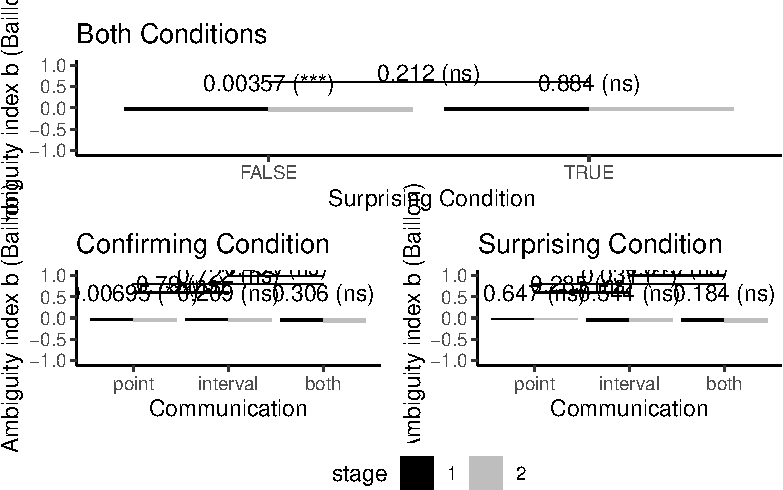
\includegraphics{03-figures_files/figure-pdf/fig-1-1.pdf}

}

\caption{\label{fig-1}Means of ambiguity index b separated by treatments
and part 1 and part 2. P-values of Wilcoxon signed-rank test comparing
part 1 and 2 directly above the mean values. P-values of
Wilcoxon--Mann--Whitney test comparing part 2 of different treatments at
the top. Note: ∗p\textless0.10, ∗∗p\textless0.05, ∗∗∗p\textless0.01, ns:
not significant}

\end{figure}

\hypertarget{figure-2}{%
\section{Figure 2}\label{figure-2}}

Next, we use the wrapper function again but visualize another outcome
using the \texttt{response\ ==\ a} argument.

\begin{figure}

{\centering 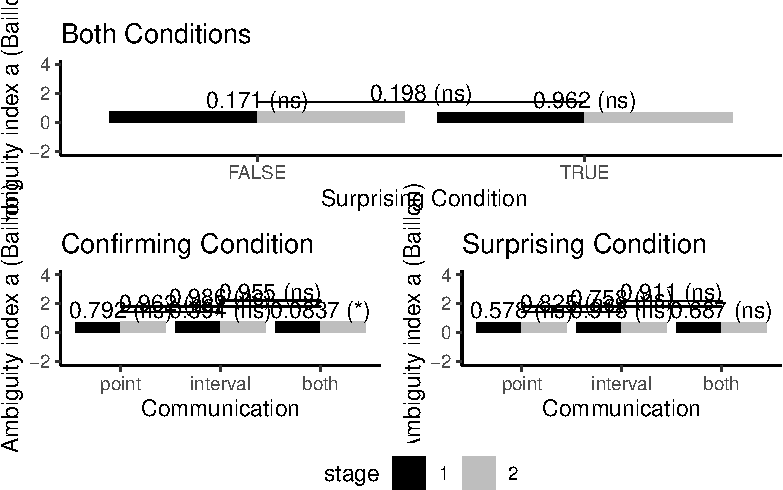
\includegraphics{03-figures_files/figure-pdf/fig-2-1.pdf}

}

\caption{\label{fig-2}Means of ambiguity index a separated by treatments
and part 1 and part 2. P-values of Wilcoxon signed-rank test comparing
part 1 and 2 directly above the mean values. P-values of
Wilcoxon--Mann--Whitney test comparing part 2 of different treatments at
the top. Note: ∗p\textless0.10, ∗∗p\textless0.05, ∗∗∗p\textless0.01, ns:
not significant}

\end{figure}

\hypertarget{figure-3}{%
\section{Figure 3}\label{figure-3}}

Figure~\ref{fig-3} also presents three panels. In contrast to
Figure~\ref{fig-1} and Figure~\ref{fig-2}, these panels visualize
confidence intervals of our estimator of interest: the interaction of
\texttt{stage} and \texttt{surprise} (top panel) as well as the
interaction between \texttt{stage} and \texttt{communication} in the
lower two panels.

The corresponding data stems from many OLS regressions and are computed
in for-loops. Even though the code differs slightly, it is very
repetitive between the three panels, which is why we only explain the
top panel

\hypertarget{top-panel}{%
\subsection{Top Panel}\label{top-panel}}

Before calculating the data based on OLS regressions, we specify three
different models: \texttt{none} represents only treatment variables,
\texttt{demographics} extends the former by adding demographic
variables, and \texttt{all} extends the former two by also adding all
remaining covariates.

Next, we run a nested loop that iterates through all three models and
within these models through both ambiguity indices \texttt{a} and
\texttt{b}. From these ols regressions, we compute clustered standard
errors using the \texttt{\{\{sandwich\}\}} and \texttt{\{\{lmtest\}\}}
package. The resuling data is stored in a temporary data.table that is
appended to an initially empty data.table called \texttt{ci\_top}.

The result looks as follows. The data.table provides a column for the
2.5\% and 97.5\% confidence interval, the center of the two, as well as
the ols specification as presented in \texttt{model} and
\texttt{outcome}.

\begin{longtable}[]{@{}rrllr@{}}
\toprule\noalign{}
2.5 \% & 97.5 \% & model & outcome & center \\
\midrule\noalign{}
\endhead
\bottomrule\noalign{}
\endlastfoot
-0.0461365 & 0.0608289 & none & a & 0.0073462 \\
-0.0085981 & 0.0374200 & none & b & 0.0144110 \\
-0.0370710 & 0.0733050 & demographics & a & 0.0181170 \\
-0.0071204 & 0.0418846 & demographics & b & 0.0173821 \\
-0.0371322 & 0.0733663 & all & a & 0.0181170 \\
-0.0071476 & 0.0419118 & all & b & 0.0173821 \\
\end{longtable}

Finally, we plot this data set (\texttt{ci\_top}) using the
\texttt{\{\{ggplot2\}\}} package. The resulting object is stored as
\texttt{top} and will be assembled together with the other two panels.

\hypertarget{left-panel}{%
\subsection{Left Panel}\label{left-panel}}

\begin{longtable}[]{@{}rrllr@{}}
\toprule\noalign{}
2.5 \% & 97.5 \% & model & outcome & center \\
\midrule\noalign{}
\endhead
\bottomrule\noalign{}
\endlastfoot
-0.1231424 & 0.0699195 & none & a (interval) & -0.0266115 \\
-0.1603397 & 0.0317751 & none & a (both) & -0.0642823 \\
-0.0085202 & 0.0705807 & none & b (interval) & 0.0310303 \\
-0.0069006 & 0.0744238 & none & b (both) & 0.0337616 \\
-0.1032781 & 0.0924975 & demographics & a (interval) & -0.0053903 \\
-0.1519774 & 0.0393496 & demographics & a (both) & -0.0563139 \\
-0.0106052 & 0.0750051 & demographics & b (interval) & 0.0321999 \\
\end{longtable}

\hypertarget{right-panel}{%
\subsection{Right Panel}\label{right-panel}}

\begin{longtable}[]{@{}rrllr@{}}
\toprule\noalign{}
2.5 \% & 97.5 \% & model & outcome & center \\
\midrule\noalign{}
\endhead
\bottomrule\noalign{}
\endlastfoot
-0.0664967 & 0.1147544 & none & a (interval) & 0.0241288 \\
-0.0495534 & 0.1325661 & none & a (both) & 0.0415063 \\
-0.0339037 & 0.0457592 & none & b (interval) & 0.0059278 \\
-0.0619626 & 0.0165198 & none & b (both) & -0.0227214 \\
-0.0798350 & 0.1115715 & demographics & a (interval) & 0.0158682 \\
-0.0675663 & 0.1267932 & demographics & a (both) & 0.0296134 \\
-0.0490060 & 0.0352795 & demographics & b (interval) & -0.0068632 \\
\end{longtable}

\hypertarget{assemble-top-left-and-right-panels}{%
\subsection{Assemble Top, Left and Right
Panels}\label{assemble-top-left-and-right-panels}}

As before, we use the \texttt{\{\{patchwork\}\}} package to assmble the
plot objects.

\begin{figure}

{\centering 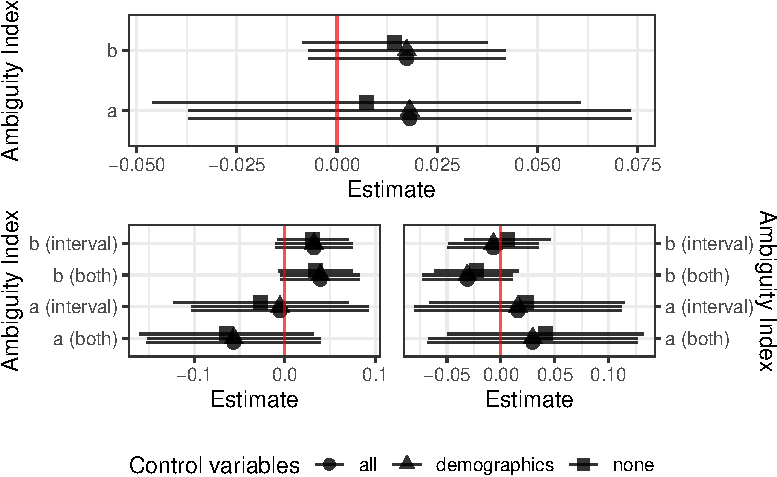
\includegraphics{03-figures_files/figure-pdf/fig-3-1.pdf}

}

\caption{\label{fig-3}Treatment effects of regression equation (1) with
dependent variables b and a. Estimators with 95\% confidence intervals.
The underlying standard errors (``HC1'') are clustered at the individual
level and estimated with the R package sandwich (Zeileis, 2004; Zeileis
et al., 2020).}

\end{figure}

\hypertarget{figure-4}{%
\section{Figure 4}\label{figure-4}}

The process of producing Figure~\ref{fig-4} is very similar to the
process of Figure~\ref{fig-3}. The only difference is that we do not
loop through the outcomes \texttt{a} and \texttt{b} but the events'
matching probabilities (\texttt{E1}, \texttt{E2}, \texttt{...},
\texttt{E23}).

To loop through these variables, we use a regex
(\texttt{E\textbackslash{}\textbackslash{}d}) to create a vector called
\texttt{events}.

Because the process is, from now on, so similar to the process of
Figure~\ref{fig-3}, we do not comment it any further here.

\hypertarget{top-panel-1}{%
\subsection{Top Panel}\label{top-panel-1}}

\begin{longtable}[]{@{}rrllr@{}}
\toprule\noalign{}
2.5 \% & 97.5 \% & model & outcome & center \\
\midrule\noalign{}
\endhead
\bottomrule\noalign{}
\endlastfoot
4.983983 & 10.142448 & none & E1 & 7.563215 \\
1.600247 & 6.299091 & none & E12 & 3.949669 \\
1.327104 & 6.115620 & none & E13 & 3.721362 \\
-7.842483 & -3.429947 & none & E2 & -5.636215 \\
-12.800137 & -7.599836 & none & E23 & -10.199987 \\
-6.107878 & -1.334793 & none & E3 & -3.721335 \\
4.421240 & 9.844463 & demographics & E1 & 7.132852 \\
\end{longtable}

\hypertarget{left-panel-1}{%
\subsection{Left Panel}\label{left-panel-1}}

\begin{longtable}[]{@{}rrllr@{}}
\toprule\noalign{}
2.5 \% & 97.5 \% & model & outcome & center \\
\midrule\noalign{}
\endhead
\bottomrule\noalign{}
\endlastfoot
-6.746653 & 1.5693594 & none & E1 (interval) & -2.5886468 \\
-7.472010 & 0.5541086 & none & E1 (both) & -3.4589505 \\
-7.466795 & 0.4839339 & none & E12 (interval) & -3.4914306 \\
-4.297893 & 3.4859217 & none & E12 (both) & -0.4059856 \\
-2.758720 & 5.5611888 & none & E13 (interval) & 1.4012346 \\
-6.134510 & 2.0764806 & none & E13 (both) & -2.0290148 \\
-4.899051 & 2.4400333 & none & E2 (interval) & -1.2295086 \\
\end{longtable}

\hypertarget{right-panel-1}{%
\subsection{Right Panel}\label{right-panel-1}}

\begin{longtable}[]{@{}rrllr@{}}
\toprule\noalign{}
2.5 \% & 97.5 \% & model & outcome & center \\
\midrule\noalign{}
\endhead
\bottomrule\noalign{}
\endlastfoot
-9.6135941 & -0.0515961 & none & E1 (interval) & -4.8325951 \\
-2.8115517 & 7.0630438 & none & E1 (both) & 2.1257460 \\
-4.0358433 & 4.3361386 & none & E12 (interval) & 0.1501477 \\
-0.4741903 & 8.1055554 & none & E12 (both) & 3.8156825 \\
-8.3619000 & -0.3107652 & none & E13 (interval) & -4.3363326 \\
-6.0444150 & 2.5918118 & none & E13 (both) & -1.7263016 \\
-1.4998061 & 6.0782483 & none & E2 (interval) & 2.2892211 \\
\end{longtable}

\hypertarget{assemble-top-left-and-right-panels-1}{%
\subsection{Assemble Top, Left and Right
Panels}\label{assemble-top-left-and-right-panels-1}}

\begin{figure}

{\centering 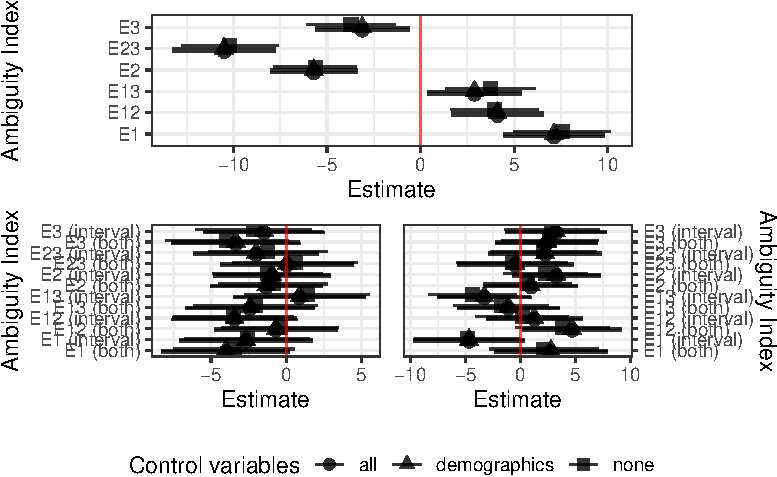
\includegraphics{03-figures_files/figure-pdf/fig-4-1.pdf}

}

\caption{\label{fig-4}Treatment effects of regression equation (1) with
matching probabilities for all events as depen- dent variables.
Estimators with 95\% confidence intervals. The underlying standard
errors (``HC1'') are clustered at the individual level and estimated
with the R package sandwich (Zeileis, 2004; Zeileis et al., 2020).}

\end{figure}

\bookmarksetup{startatroot}

\hypertarget{references}{%
\chapter*{References}\label{references}}
\addcontentsline{toc}{chapter}{References}

\markboth{References}{References}

\hypertarget{refs}{}
\begin{CSLReferences}{1}{0}
\leavevmode\vadjust pre{\hypertarget{ref-AnantanasuwongEtAl_2019}{}}%
Anantanasuwong, Kanin, Roy Kouwenberg, Olivia S Mitchell, and Kim
Peijnenberg. 2019. {``Ambiguity Attitudes about Investments: Evidence
from the Field.''} Working Paper 25561. Working Paper Series. National
Bureau of Economic Research. \url{https://doi.org/10.3386/w25561}.

\leavevmode\vadjust pre{\hypertarget{ref-Baillon_2018a}{}}%
Baillon, Aurélien, Zhenxing Huang, Asli Selim, and Peter P. Wakker.
2018. {``Measuring Ambiguity Attitudes for All (Natural) Events.''}
\emph{Econometrica} 86 (5): 1839--58.
\url{https://doi.org/10.3982/ECTA14370}.

\leavevmode\vadjust pre{\hypertarget{ref-oTree}{}}%
Chen, Daniel L., Martin Schonger, and Chris Wickens. 2016. {``oTree-an
Open-Source Platform for Laboratory, Online, and Field Experiments.''}
\emph{Journal of Behavioral and Experimental Finance} 9: 88--97.
\url{https://doi.org/10.1016/j.jbef.2015.12.001}.

\leavevmode\vadjust pre{\hypertarget{ref-Knuth_1984}{}}%
Knuth, Donald E. 1984. {``Literate Programming.''} \emph{Comput. J.} 27
(2): 97--111. \url{https://doi.org/10.1093/comjnl/27.2.97}.

\end{CSLReferences}

\cleardoublepage
\phantomsection
\addcontentsline{toc}{part}{Appendices}
\appendix

\hypertarget{session-info}{%
\chapter{Session Info}\label{session-info}}

\begin{verbatim}
R version 4.3.1 (2023-06-16)
Platform: x86_64-apple-darwin20 (64-bit)
Running under: macOS Sonoma 14.4.1

Matrix products: default
BLAS:   /Library/Frameworks/R.framework/Versions/4.3-x86_64/Resources/lib/libRblas.0.dylib 
LAPACK: /Library/Frameworks/R.framework/Versions/4.3-x86_64/Resources/lib/libRlapack.dylib;  LAPACK version 3.11.0

locale:
[1] en_US.UTF-8/en_US.UTF-8/en_US.UTF-8/C/en_US.UTF-8/en_US.UTF-8

time zone: Europe/Berlin
tzcode source: internal

attached base packages:
[1] stats     graphics  grDevices utils     datasets  methods   base     

loaded via a namespace (and not attached):
 [1] compiler_4.3.1    fastmap_1.1.1     cli_3.6.1         tools_4.3.1      
 [5] htmltools_0.5.7   rstudioapi_0.15.0 rmarkdown_2.25    knitr_1.44       
 [9] jsonlite_1.8.7    xfun_0.40         digest_0.6.33     rlang_1.1.1      
[13] evaluate_0.21    
\end{verbatim}



\end{document}
